
%----------------------------------------------------------------------------------------
%	PACKAGES AND OTHER DOCUMENT CONFIGURATIONS
%----------------------------------------------------------------------------------------

\documentclass[30pt,a0,portrait]{a0poster}
\usepackage{multicol} % This is so we can have multiple columns of text side-by-side
\columnsep=100pt % This is the amount of white space between the columns in the poster
\columnseprule=3pt % This is the thickness of the black line between the columns in the poster

\usepackage{babelbib}

\usepackage[svgnames]{xcolor} % Specify colors by their 'svgnames', for a full list of all colors available see here: http://www.latextemplates.com/svgnames-colors

\usepackage{times} % Use the times font
%\usepackage{palatino} % Uncomment to use the Palatino font
\usepackage{amsmath}
\usepackage{graphicx} % Required for including images
\graphicspath{{figures/}} % Location of the graphics files
\usepackage{booktabs} % Top and bottom rules for table
\usepackage[font=small,labelfont=bf]{caption} % Required for specifying captions to tables and figures
\usepackage{amsfonts, amsmath, amsthm, amssymb} % For math fonts, symbols and environments
\usepackage{wrapfig} % Allows wrapping text around tables and figures

\begin{document}

%----------------------------------------------------------------------------------------
%	POSTER HEADER 
%----------------------------------------------------------------------------------------

% The header is divided into two boxes:
% The first is 75% wide and houses the title, subtitle, names, university/organization and contact information
% The second is 25% wide and houses a logo for your university/organization or a photo of you
% The widths of these boxes can be easily edited to accommodate your content as you see fit
\\\\\\\
\noindent\begin{minipage}[b]{0.75\linewidth}
\veryHuge \color{Maroon} \textbf{Eternity Numbers} \color{Black}\\ % Title
\Huge\textit{The Universal Parabolic Constant}\\[2cm] % Subtitle
\huge \textbf{Ali Zafar Iqbal}\\[0.5cm] % Author(s)
\huge Concordia University, Department of Computer Science\\[0.4cm] % University/organization
\Large \texttt{Software Requirements Specifications, SOEN 6481} --- Group 5,\\
\end{minipage}
%
\begin{minipage}[b]{0.8\linewidth}

\includegraphics[scale=0.3]{figures/concordia.jpg}
\end{minipage}

\vspace{5cm} % A bit of extra whitespace between the header and poster content

%----------------------------------------------------------------------------------------

\begin{multicols}{2} % This is how many columns your poster will be broken into, a portrait poster is generally split into 2 columns


%----------------------------------------------------------------------------------------
%	INTRODUCTION
%----------------------------------------------------------------------------------------

\color{Black}
\section*{Project Focus}
\noindent The primary focus of this project was an exploratory study of a unique irrational constant (The Universal Parabolic Constant), its use in society and finally its structured implementation process as into its unique form of calculator.This project poster will confer a through analysis about the number's comprehensive background and its overall work flow.
\\

\\\noindent The inception of this project started with an understanding about the problem domain of the Universal parabolic calculator, after a initial analysis and personification of the potential users of the Universal Parabolic calculator, a formal project interview was conducted to understand and solidify the target requirements for the project's calculator which allowed the creation of a concrete Domain Modal for the Calculator \\ 

\noindent After the requirements gathering phase, the project user stories were simulated as per the original requirements and traced to their original sources for clarification purposes. 4 User stories were implemented finally in the full calculator which contained all of the basic calculations of arithmetic functions like in a normal calculator, as well as the additional functions utilizing the Universal Parabolic constant. Such as the calculation the average distance from the arc of the parabola. 
\hfill\break

\\\noindent \textbf{Deadline and milestones}\\\\
Too keep everything up to speed, the project utilized the use of multiple progress milestones, to push sprints faster. this almost became like an motivational carrot for the course. and allowed the project to be run along side the tight deadlines of the course's outer .
\hfill
\\
\\\textbf{Constant introduction}\\\\
\quad The Universal Parabolic Constant was the mathematical constant assigned for implementation during this project.  it is a type of irrational number ,defined as the ratio, for any parabola or Semicircle, of the arc length of the parabolic segment formed by the Latus-rectum to the focal parameter (Two time the focal length), it is donated by the Constant letter "P",The following is the constant's proof equation.

\hfill
 \begin{equation}
    {P=\ln(1+{\sqrt {2}})+{\sqrt {2}}=2.29558714939\dots }
\end{equation}
\begin{center}
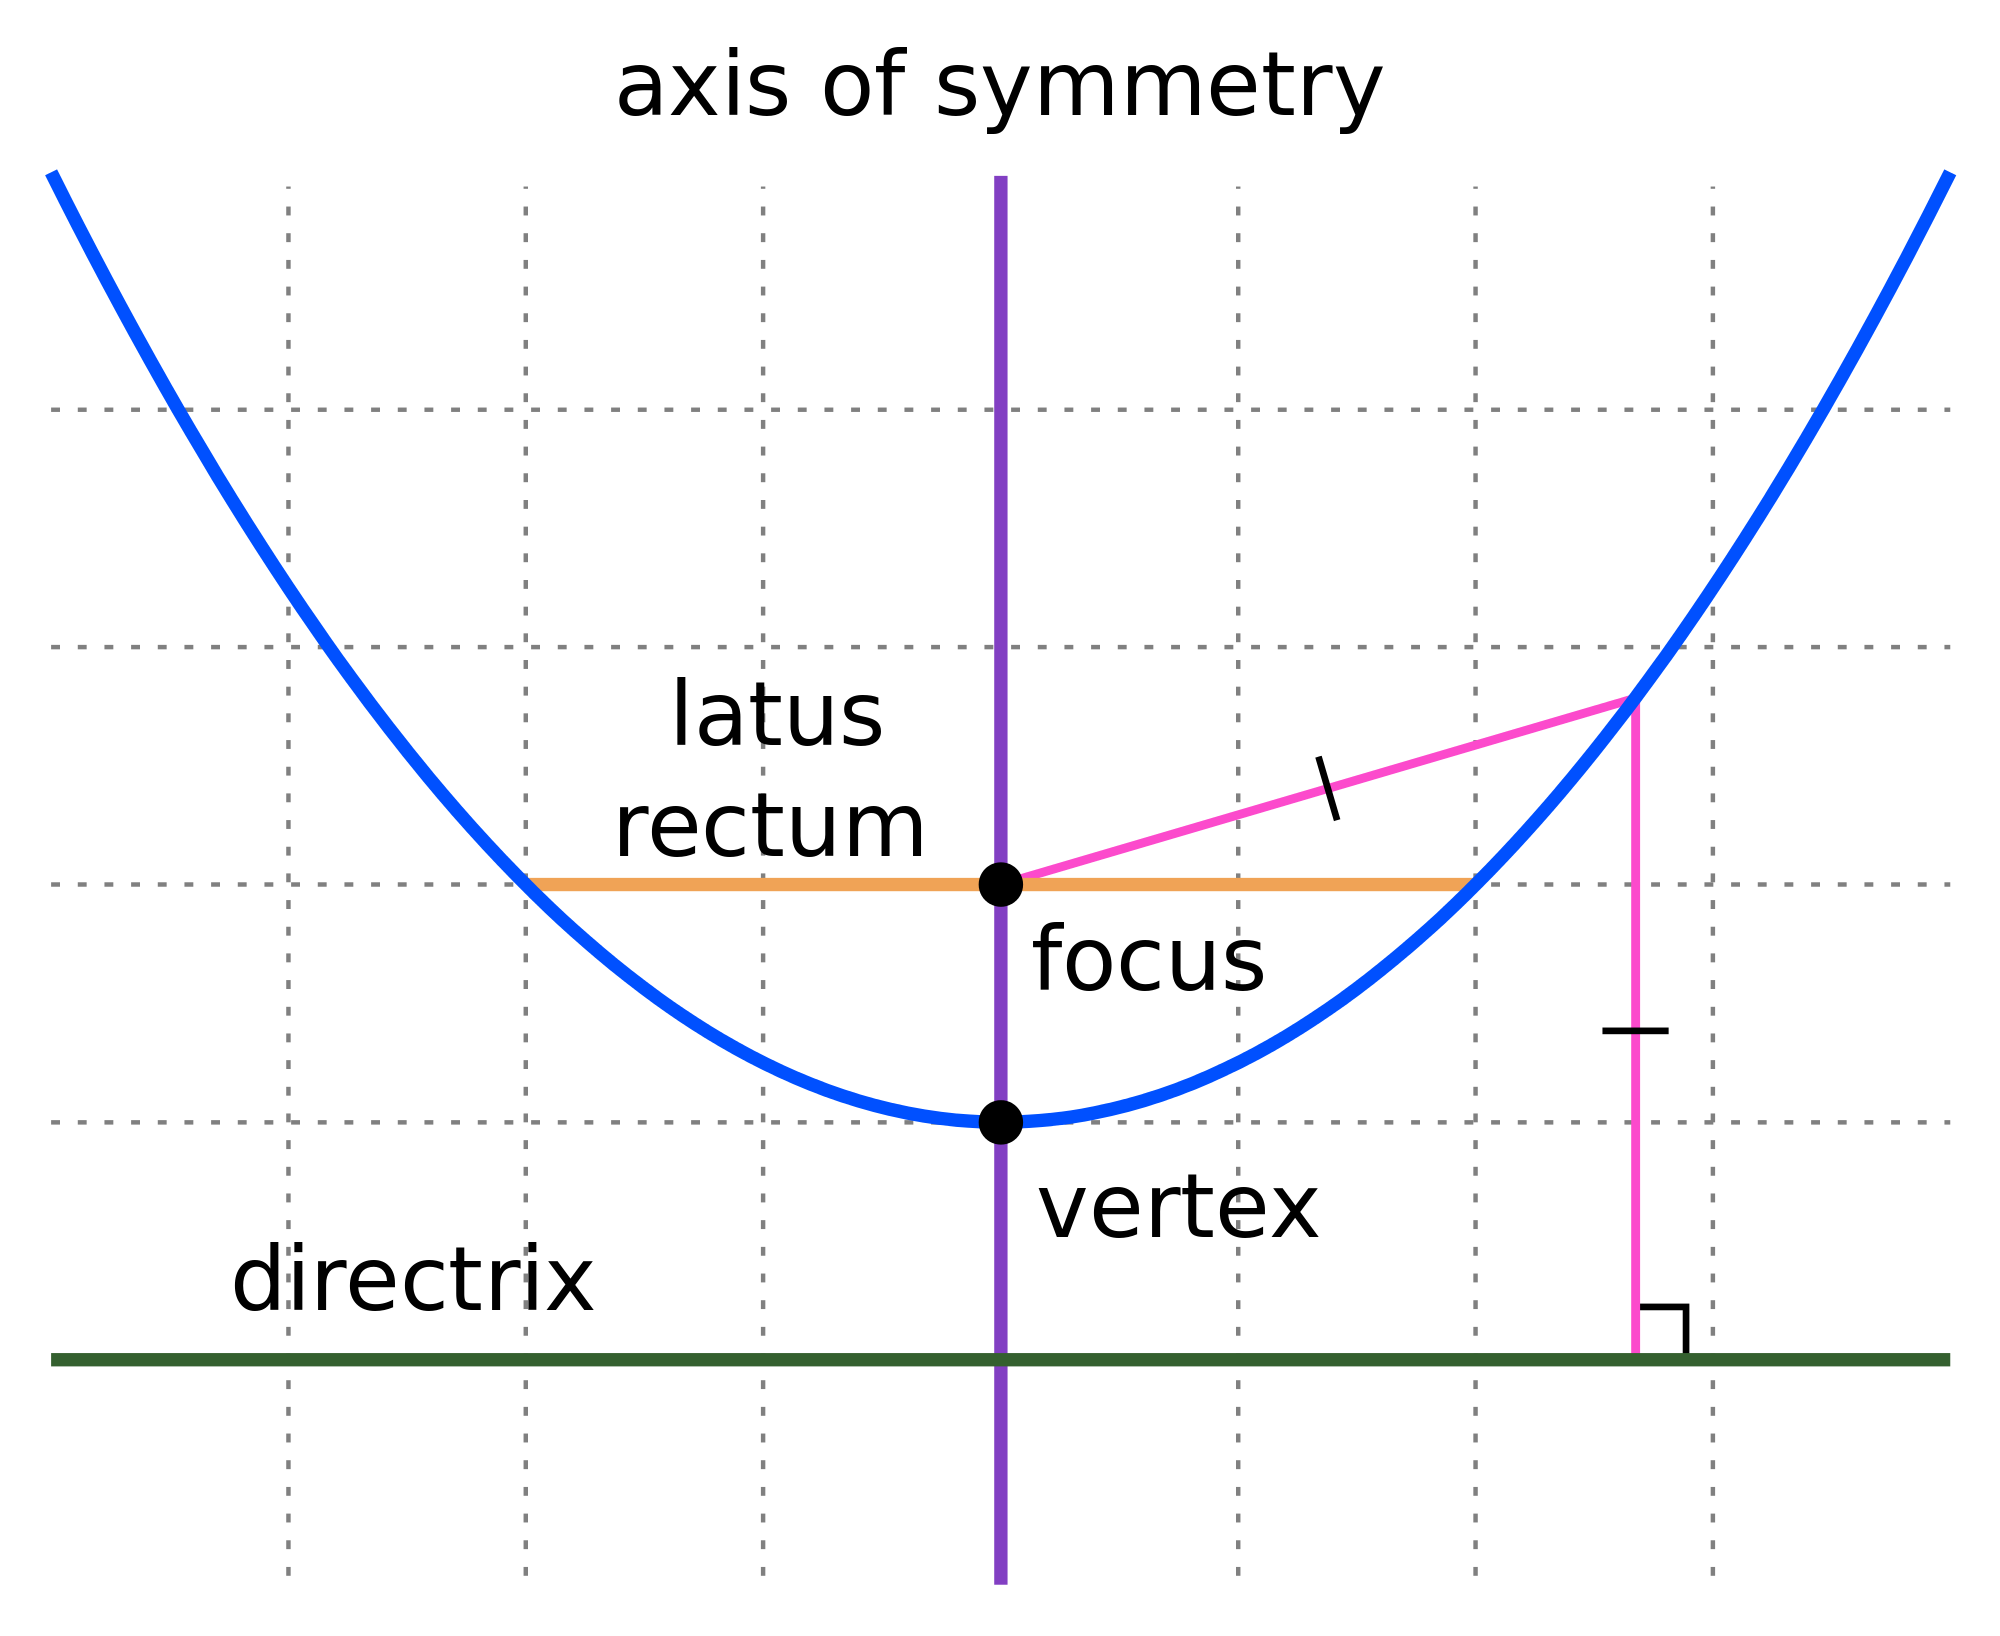
\includegraphics[scale=0.5]{figures/parabola.png}
\captionof{figure}{ An image of the latus Rectum, (The Arc length) }
\end{center}

\noindent \textbf {Applications for The Universal Parabolic Constant.}
\hfill\\\\
\noindent Universal Parabolic Constant can be used to calculate the average distance from a random point in the square unit to the center of the parabola. This can be used to measure practical distances during the constitution of real world objects such as Satellite Dishes where Incoming waves are concentrated on a singular focal point. Or architectural arcs where the extreme of arcs may need accurate points of measurements for their constructions \\

\noindent  The Universal Parabolic constant allows the creations and measurements of modern architectural structures that rely on smooth overlay curvatures as their primary foundations which are quite hard to calculate based on 3d modelling alone. an example of such structure can be seen in the following picture.

%----------------------------------------------------------------------------------------
%	OBJECTIVES
%----------------------------------------------------------------------------------------
\begin{center}\vspace{0.5cm}
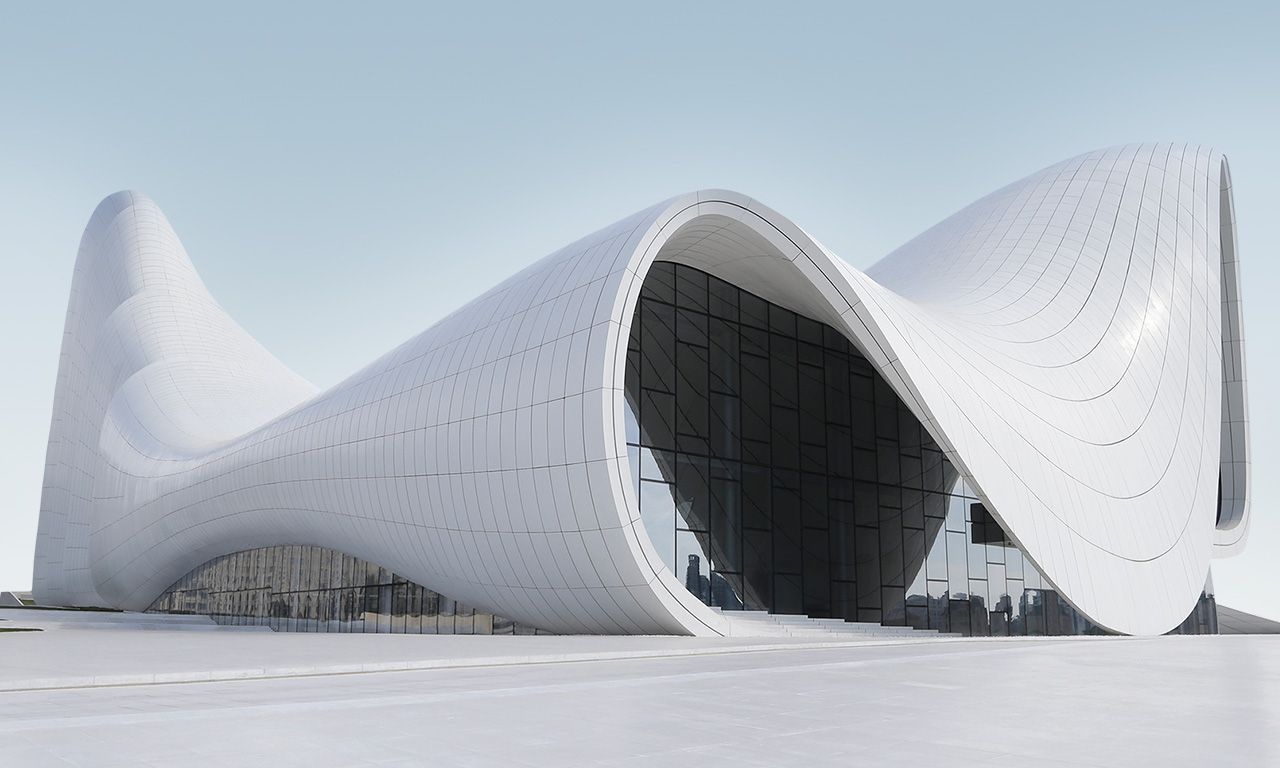
\includegraphics[width=1\linewidth]{figures/arc.jpg}
\captionof{figure}{ A modern architectural structure utilizing parabolic curvatures }
\end{center}\vspace{1cm}


\section*{Critical Decisions}
\\\\
\noindent \textbf{A Momento Implementation}\hfi \\ 

\noindent During the implementation stage of the project, A Momento design pattern was utilized for the implementation of the calculator, this choice for this design pattern was considered due the future re usability and maintainability of the calculator in the long run,As well as to perform faster Unit testing on the individual functions of the calculator during the testing phase of the project. allowing further perseverance of time for other 
\\
\\
\textbf{The Choice of Team Collaboration Tools}.\hfill \\
\\
\noindent As this project was focused around a loosely coupled team dynamic, the use of collaboration tools such as \textbf{“Figma”} and \textbf{“oMind”} allowing for live collaboration during sequential Mindmapping and target user personification playing a quintessential role to increase team productivity and collaboration, this decision was taken as time was a critical commodity that need to be managed hence, The use of these tools allowed the team to elevate loss of time by consolidation of  user personification documents and project mind maps in a singular location where they all could be worked on co collaboratively in real time. 



%----------------------------------------------------------------------------------------
%	MATERIALS AND METHODS
%----------------------------------------------------------------------------------------

\section*{Challenges}

\noindent \textbf{A Unique form of Domain}\\

\noindent The Universal Parabolic Constant was part of a unique domain area of mathematical constants, which required eccentric investigation to figure out. This was due to the fact that this domain area was really foreign in nature,  as the universal parabolic constant is used by a very niche community of people around the world.\\

\noindent \textbf{Interviewee Selections}\\

\noindent One of the Challenges faced during course of this project was the finding and arrangement of the project's formal interviewee, as stated before since the domain of mathematical constant was a foreign topic. Finding a person with experience in the field of utilizing a certain niche mathematical constant was a cumbersome experience, due to the time contains. \\

\noindent \textbf {Implementation without using the math functions.}\\

\noindent With the advent of Java and its luxuries of high level programming, the .math functions is one of the go to libraries to utilize in a scenario where mathematical functions or equations are involved, however, as one of the project constraints, the use of the .math Java library was not allowed therefore functions such as Square root and Natural logarithms had to be implemented from scratch which was daunting to understand and implement within the project's short duration.



%----------------------------------------------------------------------------------------
%	CONCLUSIONS
%----------------------------------------------------------------------------------------

\section*{Lessons Learned}

\begin{itemize}
\item Due to the intensity of the project's deadlines within a short time span, this project allowed me to better comprehend time management skills and workflow discipline which allowed me to meet those deadlines within their time frames. 

\item The project allowed me to understand the importance of software architecture, and why certain architectural styles allow are used over others. based on the overall requirements of the project.

\item Due to the content of this course and the project's topic area, This project gave an more indepth light to the idea of Ambiguity in requirements engineering and how certain non intrusive requirements can become huge bottleneck If they are left unclarified. 

\item During the Modelling stages of the project. the project allowed me to comprehend the disciplines of different requirements modellings. and why certain requirement modals have more pragmatic values over others 


\end{itemize}


%\nocite{*} % Print all references regardless of whether they were cited in the poster or not
%\bibliographystyle{plain} % Plain referencing style
%\bibliography{sample} % Use the example bibliography file %sample.bib



\end{multicols}
\end{document}